The goal of the analysis is to search for a direct indication of \gls{LFV} in the decay of Z bosons using data from proton-proton collisions measured at \gls{CMS}. Two kinds of process have to be analyzed. The first process is the signal process of the \gls{LFV} decaying Z boson. The second process are background processes of the \gls{SM} leaving the same final state particles as the signal process. To study the differences of signal and background, both are simulated using Monte Carlo simulations (\gls{MC}). Including statistical and systematic uncertainties arising from the measurement, statistical methods are used to evaluate the simulation in comparison to data. 


\section{Signal and background processes}

\subsection{Signal process}
\label{sec:section_3_1_1}

To violate lepton flavour, the individual sum of each lepton flavour in initial and final state must be different: 

\begin{equation}
	\label{eq:eq_3_1}
	\sum_{n \text{ initial state particle}} f_{n} \neq  \sum_{n \text{ final state particle}} f_{n}
\end{equation}

In the case of a Z boson, produced via quark annihilation in a proton proton collider, three possible configurations fulfil the condition. The direct decay of a Z boson into an electron and a muon, referred to as $e\mu$ final state, into an electron and a $\tau$ lepton, referred to as $e\tau$ final state, or into a muon and a $\tau$ lepton, referred to as $\mu\tau$ final state, violates lepton flavour. The feynman diagrams of these processes are shown in figure \ref{fig:fig_3_1}. \\

\begin{figure}[htp]
	\centering

	\begin{tikzpicture}[node distance=1.5cm]
		\coordinate[label=left:$q$] (q1);
		\coordinate[below=3cm of q1, label=left:$q$] (q2);
   
		\coordinate[below =1.5cm of q1] (k1); \coordinate[right =1.5cm of k1] (v1); 
		\coordinate[right =2cm of v1] (v2); \coordinate[right =1.5cm of v2] (k2);
		
		\coordinate[above=1.5 cm of k2,label=right:$e$] (l1);
		\coordinate[below=3cm of l1, label=right:$\mu$] (l2);

		\draw[fermion] (q1) -- (v1);
		\draw[fermion] (v1) -- (q2);
		\draw[photon] (v1) -- node[label=above:$Z$] {} (v2);
		\draw[fermion] (l1) -- (v2);
		\draw[fermion] (v2) -- (l2);
	\end{tikzpicture}

	\begin{tikzpicture}[node distance=1.5cm]
		\coordinate[label=left:$q$] (q1);
		\coordinate[below=3cm of q1, label=left:$q$] (q2);
   
		\coordinate[below =1.5cm of q1] (k1); \coordinate[right =1.5cm of k1] (v1); 
		\coordinate[right =2cm of v1] (v2); \coordinate[right =1.5cm of v2] (k2);
		
		\coordinate[above=1.5 cm of k2,label=right:$e$] (l1);
		\coordinate[below=3cm of l1, label=right:$\tau$] (l2);

		\draw[fermion] (q1) -- (v1);
		\draw[fermion] (v1) -- (q2);
		\draw[photon] (v1) -- node[label=above:$Z$] {} (v2);
		\draw[fermion] (l1) -- (v2);
		\draw[fermion] (v2) -- (l2);
	\end{tikzpicture}

	\begin{tikzpicture}[node distance=1.5cm]
		\coordinate[label=left:$q$] (q1);
		\coordinate[below=3cm of q1, label=left:$q$] (q2);
   
		\coordinate[below =1.5cm of q1] (k1); \coordinate[right =1.5cm of k1] (v1); 
		\coordinate[right =2cm of v1] (v2); \coordinate[right =1.5cm of v2] (k2);
		
		\coordinate[above=1.5 cm of k2,label=right:$\mu$] (l1);
		\coordinate[below=3cm of l1, label=right:$\tau$] (l2);

		\draw[fermion] (q1) -- (v1);
		\draw[fermion] (v1) -- (q2);
		\draw[photon] (v1) -- node[label=above:$Z$] {} (v2);
		\draw[fermion] (l1) -- (v2);
		\draw[fermion] (v2) -- (l2);
	\end{tikzpicture}
	
	\caption[Feynman diagram of LFV Z boson decay]{Feynman diagram of LFV Z boson decay into the $e\mu$, $e\tau$ and $\mu\tau$ final state}
	\label{fig:fig_3_1}

\end{figure}

The $\tau$ lepton \cite{TAU} has a special role in comparison to electrons or muons. Due to the mean life time of 2.9$\cdot 10^{-13}$ seconds the $\tau$ lepton decays after a flight distance of a few micrometers and leaves secondary vertices in the tracker system. The $\tau$ lepton can decay leptonically with a branching ratio of $\text{BR}(\tau \to l\nu_{\tau}\nu_{l}) = 0.34$ or hadronically with a branching ratio of $\text{BR}(\tau \to \nu_{\tau} + \text{hadrons}) = 0.66$. Because of the high branching ratio of the hadronic decaying $\tau$ leptons (\gls{TAUH}), only this type of decay is considered in the content of the analysis. The \gls{TAUH} are reconstructed from jets, which originate from the hadrons of the $\tau$ decay. 

\subsection{Background processes}
\label{sec:section_3_1_2}

Background processes have the same particles in the final state as the \gls{LFV}, but they originate from leptonic/semi-leptonic decays of the mother particles or from misidentification of the particles. This leads to differences in kinematic distributions, different secondary vertices and/or additional particles in the final state beside the two leptons. \\

\subsection*{Drell Yan}

The main irreducible background is the Drell-Yan (\gls{DY}) $Z\to\tau\tau$ process, both $\tau$ leptons decays leptonically into an electron, a muon and four neutrinos, or one $\tau$ lepton decays leptonically into a lepton and the other one decays hadronically with three neutrinos. The leptons from the $\tau$ lepton decays originate from secondary vertices and have different kinematic properties in comparison to the leptons originating from \gls{LFV}. Due to the neutrinos, which carries away the momenta undetected, this process will have in general more \gls{MET} in the event compared to the \gls{LFV} process. Figure \ref{fig:fig_3_2} shows the Feynman diagram of the leptonic decay chain. Besides the $Z\to\tau\tau$ process, the second \gls{DY} process is $Z\to\ell\ell$ with $l \in (e, \mu$), where one of the leptons $\ell$ has a misidentified lepton flavour. In this case the kinematic properties are quite similar to the \gls{LFV} process, because the lepton also originate from the $Z$ boson, and have no secondary vertices or neutrinos. \\


\begin{figure}[htp]
	\centering

	\begin{tikzpicture}[node distance=1.5cm]
		\coordinate[label=left:$q$] (q1);
		\coordinate[below=3cm of q1, label=left:$q$] (q2);

		\coordinate[right =1.5cm of k1] (v1); 
		\coordinate[right =2cm of v1] (v2); \coordinate[right =1.5cm of v2] (k2);
	
		\coordinate[above=1.5 cm of k2] (tau1);
		\coordinate[below=1.5cm of k2] (tau2);
	
		\coordinate[right=1.5 cm of tau1] (k3);
		\coordinate[above=1 cm of k3, ] (W1);
		\coordinate[below=1 cm of k3,label=right:$\nu_{\tau}$] (nu1);
		\coordinate[right=1.5 cm of W1] (k4);
		\coordinate[above=1 cm of k4, label=right:$e$] (l1);
		\coordinate[below=1 cm of k4, label=right:$\nu_{e}$] (nu2);
	
		\coordinate[right=1.5 cm of tau2] (k5);
		\coordinate[above=1 cm of k5,label=right:$\nu_{\tau}$] (nu3);
		\coordinate[below=1 cm of k5] (W2);
		\coordinate[right=1.5 cm of W2] (k6);
		\coordinate[above=1 cm of k6, label=right:$\mu$] (l2);
		\coordinate[below=1 cm of k6,label=right:$\nu_{\mu}$] (nu4);
	
		\draw[fermion] (q1) -- (v1);
		\draw[fermion] (v1) -- (q2);
		\draw[photon] (v1) -- node[label=above:$Z$] {} (v2);
		\draw[fermion] (tau1) -- node[label=above:$\tau$] {} (v2);
		\draw[fermion] (v2) -- node[label=below:$\tau$] {} (tau2);
	
   		\draw[fermion] (nu1) -- (tau1);
   		\draw[photon] (tau1) -- node[label=above:$W$] {} (W1);
   		\draw[fermion] (l1) -- (W1);
   		\draw[fermion] (W1) -- (nu2);
	
   		\draw[photon] (W2) -- node[label=below:$W$] {} (tau2);
   		\draw[fermion] (tau2) -- (nu3);
   		\draw[fermion] (l2) -- (W2);
   		\draw[fermion] (W2) -- (nu4);
	\end{tikzpicture}
	
	\caption[Feynman diagram of $Z\to\tau\tau$ decay]{Feynman diagram of $Z\to\tau\tau$ fully leptonic decay in the $e\mu$ final state}
	\label{fig:fig_3_2}
\end{figure}

\subsection*{Top/anti-top production}

One of the other backgrounds is the top/anti-top production (\gls{TTBAR}), in which the top pair decays leptoncally into leptons, b-quarks and neutrinos. Figure \ref{fig:fig_3_3} shows the Feynman diagram of the leptonic decay chain. Like in the $Z\to\tau\tau$ process the leptons originate from secondary vertices and have different kinematic properties in comparison to the signal. \\


\begin{figure}[htp]
	\centering

	\begin{tikzpicture}[node distance=1.5cm]
		\coordinate[label=left:$g$] (g1);
		\coordinate[below=3cm of g1, label=left:$g$] (g2);

		\coordinate[right =1.5cm of k1] (v1); 
		\coordinate[right =2cm of v1] (v2); \coordinate[right =1.5cm of v2] (k2);
	
		\coordinate[above=1.5 cm of k2] (top1);
		\coordinate[below=1.5cm of k2] (top2);
	
		\coordinate[right=1.5 cm of tau1] (k3);
		\coordinate[above=1 cm of k3, ] (W1);
		\coordinate[below=1 cm of k3,label=right:$b$] (b1);
		\coordinate[right=1.5 cm of W1] (k4);
		\coordinate[above=1 cm of k4, label=right:$\ell$] (l1);
		\coordinate[below=1 cm of k4, label=right:$\nu_{\ell}$] (nu1);
	
		\coordinate[right=1.5 cm of tau2] (k5);
		\coordinate[above=1 cm of k5,label=right:$b$] (b2);
		\coordinate[below=1 cm of k5] (W2);
		\coordinate[right=1.5 cm of W2] (k6);
		\coordinate[above=1 cm of k6, label=right:$\ell'$] (l2);
		\coordinate[below=1 cm of k6,label=right:$\nu_{\ell'}$] (nu2);
	
		\draw[gluon] (g1) -- (v1);
		\draw[gluon] (v1) -- (g2);
		\draw[gluon] (v1) -- node[label=above:$g$] {} (v2);
		\draw[fermion] (top1) -- node[label=above:$t$] {} (v2);
		\draw[fermion] (v2) -- node[label=below:$t$] {} (top2);
	
   		\draw[fermion] (b1) -- (top1);
   		\draw[photon] (top1) -- node[label=above:$W$] {} (W1);
   		\draw[fermion] (l1) -- (W1);
   		\draw[fermion] (W1) -- (nu1);
	
   		\draw[photon] (W2) -- node[label=below:$W$] {} (top2);
   		\draw[fermion] (top2) -- (b2);
   		\draw[fermion] (l2) -- (W2);
   		\draw[fermion] (W2) -- (nu2);
	\end{tikzpicture}

	\caption[Feynman diagram of \gls{TTBAR} decay]{Feynman diagram of \gls{TTBAR} decay chain}
	\label{fig:fig_3_3}
\end{figure}

\subsection*{Di-boson}

Besides the decay of fermions like the $\tau$ leptons and the tops, also the lepton decay of a pair of vector bosons leaves to leptons. The possible vector bosons pairs are $ZZ$/$WW$/$WZ$. Figure \ref{fig:fig_3_4} shows the Feynman diagram of vector boson production. For the $WW$ pair, the $W$ bosons decay into two leptons with two neutrinos, for the $ZZ$ pair the Z bosons decay into four leptons, where two leptons are not identified correctly, and for the $WZ$ pair the bosons decay into three leptons and a neutrino, there one of the leptons is not identified correctly. \\


\begin{figure}[htp]
	\centering
	\begin{tikzpicture}[node distance=1.5cm]
		\coordinate[label=left:$q$] (q1);
		\coordinate[right=2cm of q1] (v1);
		\coordinate[below=2.5cm of v1] (v2);
		\coordinate[left=2cm of v2, label=left:$q$] (q2);
		\coordinate[right=2cm of v1] (Z1);
		\coordinate[right=2cm of v2] (Z2);
		
		\coordinate[right=1 cm of Z1] (k1);
		\coordinate[above=1 cm of k1, label=right:$\ell/\ell$] (l1);
		\coordinate[below=1 cm of k1, label=right:$\ell/\nu_{\ell}$] (l2);
		
		\coordinate[right=1 cm of Z2] (k2);
		\coordinate[above=1 cm of k2, label=right:$\ell'/\ell'$] (l3);
		\coordinate[below=1 cm of k2, label=right:$\ell'/\nu_{\ell'}$] (l4);
		
		\draw[fermion] (q1) -- (v1);
		\draw[fermion] (v1)  -- node[label=left:$q$] {} (v2);
		\draw[fermion] (v2) -- (q2);
		\draw[photon] (v1)  -- node[label=above:$Z/W$] {} (Z1);
		\draw[photon] (v2)  -- node[label=below:$Z/W$] {} (Z2);
		
		\draw[fermion] (l1) -- (Z1);
		\draw[fermion] (Z1) -- (l2);
		\draw[fermion] (l3) -- (Z2);
		\draw[fermion] (Z2) -- (l4);
	\end{tikzpicture}

	\caption[Feynman diagram of vector boson process]{Feynman diagram of vector boson process}
	\label{fig:fig_3_4}
\end{figure}

\subsection*{W + jets and \gls{QCD}}

On the other hand processes exist, in which the end state particles are not identified correctly, like discussed for the $Z\to\ell\ell$ process. One of the processes is the single $W$ boson production in association with a quark, as seen in figure \ref{fig:fig_3_5}. The $W$ boson decays leptonically, but the quark jet is misidentified as a lepton or a \gls{TAUH}. The other process are \gls{QCD} multijet processes, which are the result of the hard interaction of the partons from the protons. These processes lead to quarks/gluons in the final state, which jets are then misidentified as leptons. Figure  \ref{fig:fig_3_6} shows two possible Feynman diagrams contributing to the \gls{QCD} background. \\

\begin{figure}[htp]
	\centering
	\begin{tikzpicture}[node distance=1.5cm]
		\coordinate[label=left:$g$] (g);
		\coordinate[below=3cm of g, label=left:$q$] (q1);
		
		\coordinate[right=2cm of g] (k);
		\coordinate[below=1cm of k] (v1);
		\coordinate[below=1cm of v1] (v2);
		
		\coordinate[right=4cm of g, label=right:$q'$] (q3);
		\coordinate[right=4cm of q1] (W);

		\coordinate[right=1cm of W] (k2);
		\coordinate[above=1cm of k2, label=right:$\ell$] (l);
		\coordinate[below=1cm of k2, label=right:$\nu_{\ell}$] (nu);
		
		\draw[gluon] (g) -- (v1);
		\draw[fermion] (q1) -- (v2);
		\draw[fermion] (v2) -- node[label=right:$q'$] {} (v1);
		\draw[fermion] (v1) -- (q3);
		\draw[photon] (v2) -- node[label=below:$W$] {} (W);

		\draw[fermion] (nu) -- (W);
		\draw[fermion] (W) -- (l); 
	\end{tikzpicture}

	\caption[Feynman diagram of $W + \text{jets}$ process]{Feynman diagram of $W + \text{jets}$ process}
	\label{fig:fig_3_5}
\end{figure}

\begin{figure}[htp]
		\begin{tikzpicture}[node distance=1.5cm]
			\coordinate[label=left:$g$] (g1);
			\coordinate[below=3cm of g1, label=left:$g$] (g2);   			
			\coordinate[below =1.5cm of g1] (k1); \coordinate[right =1.5cm of k1] (v1); 
			\coordinate[right =2cm of v1] (v2); \coordinate[right =1.5cm of v2] (k2);
		
			\coordinate[above=1.5 cm of k2,label=right:$q$] (q1);
			\coordinate[below=3cm of q1, label=right:$q$] (q2);
	
			\draw[gluon] (g1) -- (v1);
			\draw[gluon] (v1) -- (g2);
			\draw[gluon] (v1) -- node[label=above:$g$] {} (v2);
			\draw[fermion] (q1) -- (v2);
			\draw[fermion] (v2) -- (q2);

			\coordinate[right=3cm of q1, label=left:$q$] (2_q1);
			\coordinate[right=2cm of 2_q1] (2_v1);
			\coordinate[below=2.5cm of 2_v1] (2_v2);
			\coordinate[left=2cm of 2_v2, label=left:$q$] (2_q2);
			\coordinate[right=2cm of 2_v1] (2_g1);
			\coordinate[right=2cm of 2_v2] (2_g2);

			
			\draw[fermion] (2_q1) -- (2_v1);
			\draw[fermion] (2_v1)  -- node[label=left:$q$] {} (2_v2);
			\draw[fermion] (2_v2) -- (2_q2);
			\draw[gluon] (2_v1)  -- node[label=above:$g$] {} (2_g1);
			\draw[gluon] (2_v2)  -- node[label=below:$g$] {} (2_g2);
		\end{tikzpicture}

	
	\caption[Feynman diagram of \gls{QCD} background]{Feynman diagram of two possible contributions to the \gls{QCD} multijet background}
	\label{fig:fig_3_6}
\end{figure}


\section{Event selection}
\label{sec:section_3_2}

From all events, which are recorded by \gls{CMS}, only a fraction of them are particularly interesting regarding the search for \gls{LFV}. The search for \gls{LFV} requires events having leptons with different flavour, which are well reconstructed and isolated. Because of this, an analysis specific event selection is performed. This selection is divided into two steps. The first step is the reconstruction/identification of the objects, where the raw detector information is evaluated with specific software tools. The second step is to select the reconstructed objects of interest in specific events and to set criteria in regard to the quality of reconstruction. 


\subsection{Event reconstruction}
\label{sec:section_3_2_1}

Like discussed in section \ref{sec:section_2_2_4} and illustrated in figure \ref{fig:fig_2_5}, different particles leave specific signatures in the detector systems of \gls{CMS}. This fact is used in the particle flow algorithm (\gls{PF}) \cite{PF}. The algorithm identifies objects electrons and photon from \gls{ECAL} entries or muons from hits in the muon chambers. By linking the information of the different detector systems, for example a track in the tracker system and matching \gls{ECAL} entries, all particles can be identified one after another.  From the combination of all reconstructed particle higher level objects like jets or \gls{MET} are reconstructed. \\

To ensure the best possible identification efficiency of the reconstructed particles, the \gls{CMS} collaboration provides multivariate analysis (\gls{MVA}) classifiers for the different particles. The classifiers are trained to identify the particle of interest from other particles, where information of detector systems are fed into the training, see reference \cite{ERECO} for the electron \gls{MVA} classifier. \\

The $\tau$ leptons require more sophisticated methods for reconstruction, because of the short lifetime and the decay products of the $\tau$ lepton. The \gls{TAUH} are reconstructed with the hadron-plus-strips algorithm \cite{TAURECO}. This algorithm uses information of the tracks and calorimeter deposition of the hadrons originating from the decay of the $\tau$ lepton to a charged pion (1-prong), to a charged pion and a neutral pion (1-prong + $\pi^0$) and to three charged pions (3-prong). \\

As for other objects the \gls{CMS} collaboration provides \gls{MVA} classifier for \gls{TAUH} \cite{TAURECO}. But due to reconstruction of the \gls{TAUH} from decay products, it is more prone that other objects (in general electrons/muons/jets) are misidentified as \gls{TAUH}. For this reason three different \gls{MVA} are provided to differentiate \gls{TAUH} and electrons/muons/jets. \\

Besides $\tau$ leptons, also jets need a sophisticated treatment to be identified from a particle cascade in the calorimeter systems. Jets are reconstructed using the anti-$k_T$ algorithm \cite{ANTIKT}, which cluster all \gls{PF} candidates originating from the primary vertex within a cone of \gls{dR} = 0.4. In this analysis jets are required to fulfil \gls{pT} $> 30$ GeV and $|$\gls{eta}$|$ $ < 4.7$ to be identified as a jet. Due to the \gls{TTBAR} and its decay into b-quarks, the combined secondary vertex algorithm \cite{CSV} is used, which uses information about track-based lifetime information and the secondary vertex to provide a classifier to identify jets from b-quarks. 


\subsection{Selection criteria}
\label{sec:section_3_2_2}

For the search of \gls{LFV} in Z boson decays, events of interest contain a pair of reconstructed electron/muon, electron/tau lepton or muon/tau lepton. On these reconstructed leptons qualitative requirements are set, in order to maximize the confidence in the quality of the reconstruction. \\

The first requirement is the trigger decision of the \gls{HLT}, which is discussed in section \ref{sec:section_2_2_3}. There is not only one trigger decision, but many trigger decisions are made on the objects of interest. The decision of the trigger is based on the \gls{pT} and \gls{eta} of the particles, which are online reconstructed during the trigger decision. 

\begin{description}
	\item [$e\mu$:] In this final state two cross triggers are used, which selects events with one electron and one muon. The first trigger selects an electron with \gls{pT} $> 23$ GeV and $|$\gls{eta}$|$ $< 2.5$ and a muon with \gls{pT} $> 8$ GeV and $|$\gls{eta}$|$ $< 2.4$ and the second trigger requires an electron with \gls{pT} $> 12$ GeV and $|$\gls{eta}$|$ $< 2.5$ and a muon with \gls{pT} $> 23$ GeV and $|$\gls{eta}$|$ $< 2.4$. 
	\item [$e\tau$:] In this final state a single trigger is used to select events with electrons. The trigger requires an electron with \gls{pT} $> 25$ GeV and $|$\gls{eta}$|$ $< 2.1$
	\item [$\mu\tau$:] In this final state a single trigger for selecting events with a muon and a cross trigger for selecting a pair of muon and \gls{TAUH}. The cross trigger requires a muon with \gls{pT} $> 19$ GeV and $|$\gls{eta}$|$ $< 2.1$ and a \gls{TAUH} with \gls{pT} $> 20$ GeV and $|$\gls{eta}$|$ $< 2.5$ and the single trigger requires muons with \gls{pT} $> 22$ GeV and $|$\gls{eta}$|$ $< 2.1$.
\end{description}

The second requirement is the isolation of the leptons. The isolation quantifies the energy deposition around a reconstructed object in a cone defined by a specific value of \gls{dR}. The definition of isolation is given by

\begin{equation}
	\label{eq:eq_3_1}
	I^{\ell} = \frac{\sum_{\text{charged}} p_{T} + \text{max}(0, \sum_{\text{neutral}} p_{T} - \frac{1}{2}\sum_{\text{charged, PU}} p_{T})}{p_T^{\ell}}  
\end{equation} 

with $\sum_{\text{charged}}$ \gls{pT} as sum of the scalar transverse momenta of all charged particles originating from the primary vertex, $\sum_{\text{neutral}}$ \gls{pT} as sum of the scalar transverse momenta of all neutral particles and $\sum_{\text{charged, PU}}$ \gls{pT} as sum of the scalar transverse momenta of all charged particles from secondary vertices in a cone of \gls{dR} = 0.4. In this analysis tight isolated lepton are required, which means for each final state: 

\begin{description}
	\item [$e\mu$:] For the electron an isolation of $I^{e} \leq  0.15$ and for the muon $I^{\mu} \leq  0.2$ are required. 
	\item [$e\tau$:]  For the electron an isolation of $I^{e} \leq  0.10$ is required. For the \gls{TAUH} a \gls{MVA} ID is used for quantifying isolation, which is trained to distinguish between quark/gluon jets. 
	\item [$\mu\tau$:]  For the muon an isolation of $I^{\mu} \leq 0.10$ is required. Like in the $e\tau$ final state the \gls{TAUH} has to pass the \gls{MVA} ID for isolation.
\end{description}


The third requirement is based on the identification of the particle. To ensure that the object of interest is correctly identified, an offline criteria based on the detectors entries and particles properties are either used to set cuts on this or to train a \gls{MVA} classifier, like mentioned in section \ref{sec:section_3_2_1}. The \gls{CMS} collaboration provides recommendations for each particle, where different so-called working points for the selections are defined. These range from very loose to very tight, where a tighter working indicates a more trustworthy selection, but of course also lead to less events, which are selected. Which working point gives the best balance depends on the analysis, the following list shows the choice for this analysis. 

\begin{description}
	\item [$e\mu$:] The electron has to pass the tight \gls{MVA} identification criteria, while the muon has to pass the medium cut based identification criteria. 
	\item [$e\tau$:]  The electron has to pass the tight \gls{MVA} identification criteria, while the \gls{TAUH} has to pass the tight \gls{MVA} identification criteria to be distinguished from electrons and the loose \gls{MVA} identification criteria to be distinguished from muons.
	\item [$\mu\tau$:]  The muon has to pass the medium cut based identification criteria, while the \gls{TAUH} has to pass the loose \gls{MVA} identification criteria to be distinguished from electrons and the tight \gls{MVA} identification criteria to be distinguished from muons.
\end{description}


\subsection{Categorization}
\label{sec:section_3_2_3}

The events from signal and background processes differ in their kinematics properties. This fact can be used in the statistical interpretation of the analysis, see section \ref{sec:section_5_2}. A categorization of the phase space is applied, which defines different region of interest. \\

In this analysis the number of jets are of interest. As discussed in section \ref{sec:section_3_1_2}, the \gls{LFV} signal leads always to leptons with different flavour. There are two possible sources of jets for signal events. One source are jets, which are radiated from quarks before their annihilation to the Z boson. The other source of jets in the final state are quarks/gluons coming from the other constituents of the proton. The same argumentation is also true for the \gls{DY} background. This leads to a distribution, where most events have zero jets and the number of jets in events is expected to be smaller for each additional jet. In comparison, some background processes have always jets in their final state. Backgrounds like \gls{TTBAR}, W + jets and \gls{QCD} multijet have jets in the final state because of the properties of the interaction or the decay of the final state particles, as discussed in section \ref{sec:section_3_1_2}. The described jet distributions are shown in figure \ref{fig:fig_3_7}. \\

\begin{figure}[htp]
	\centering
	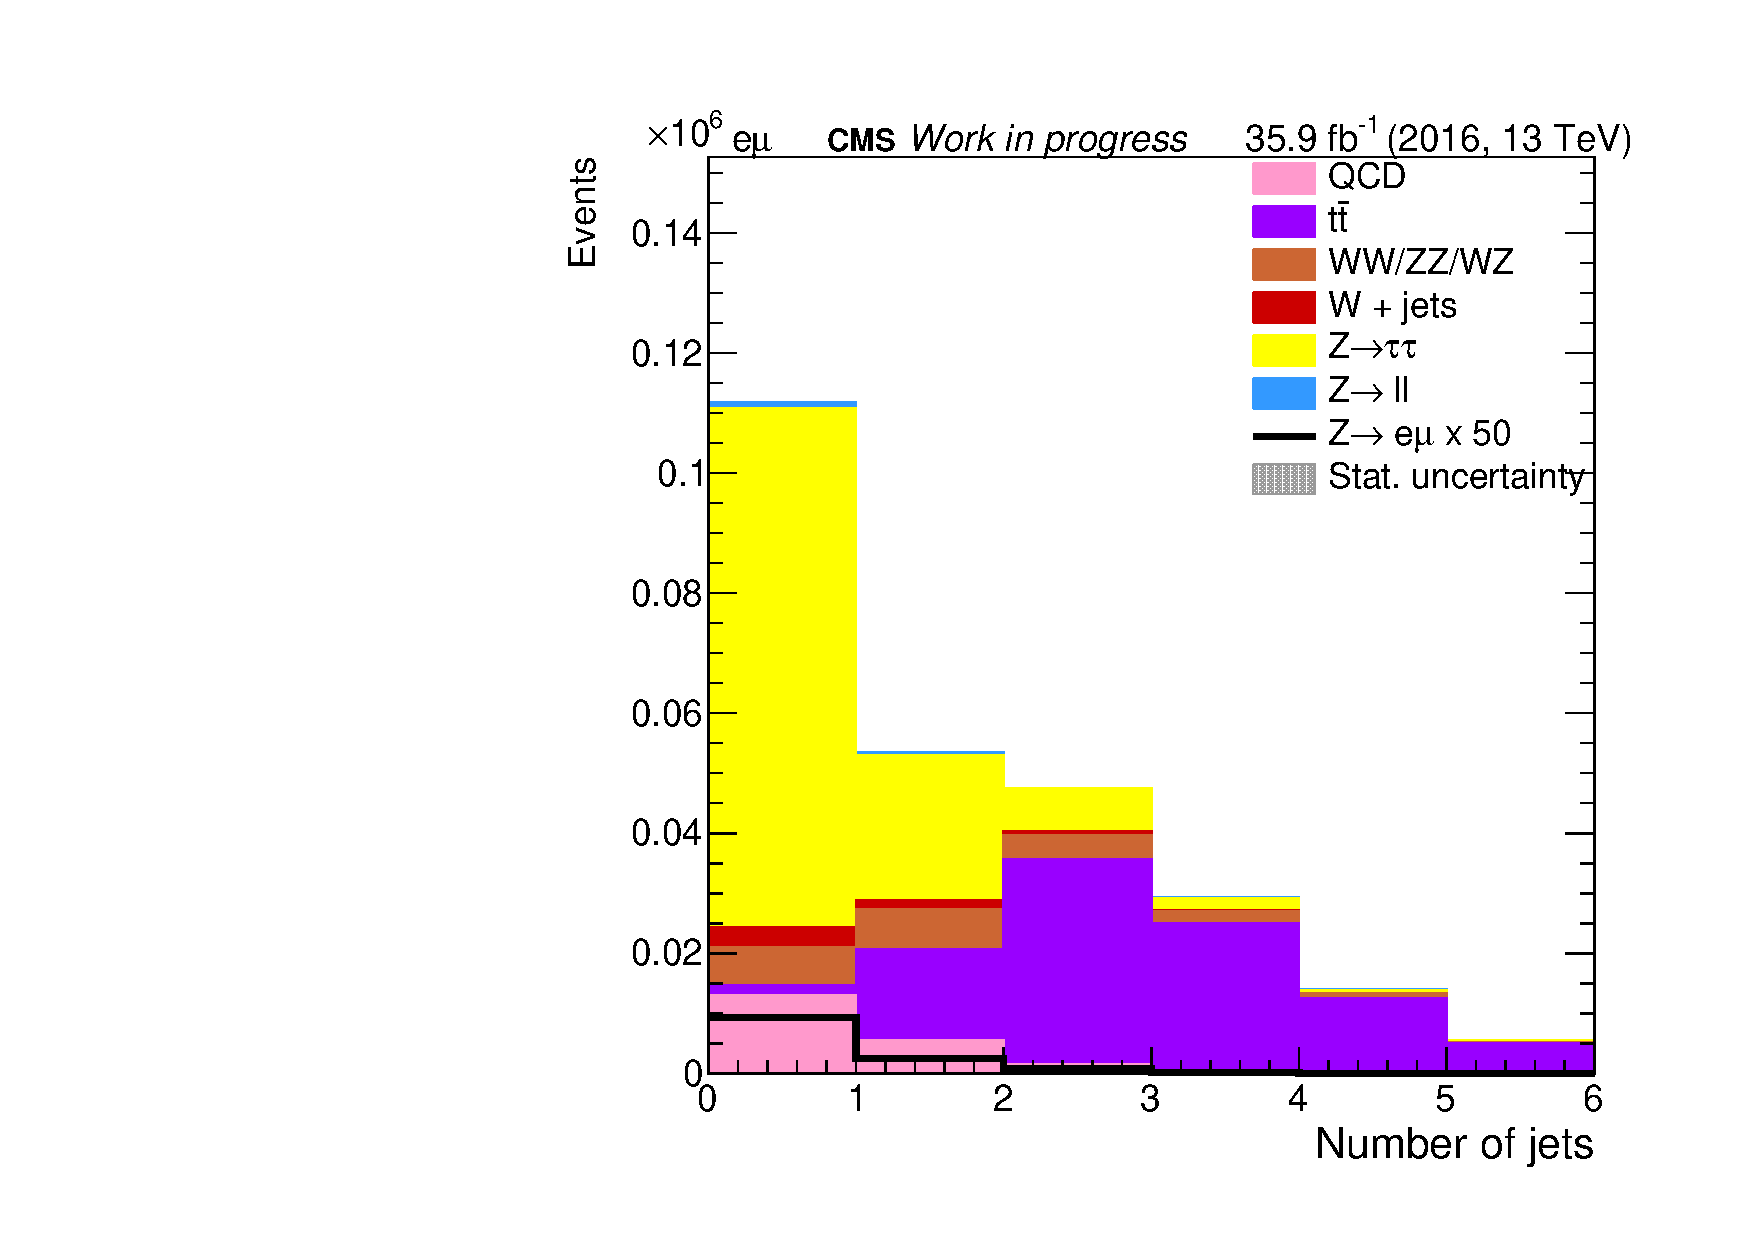
\includegraphics[width=0.55\textwidth]{plots/em/NumberOfJets.pdf}
	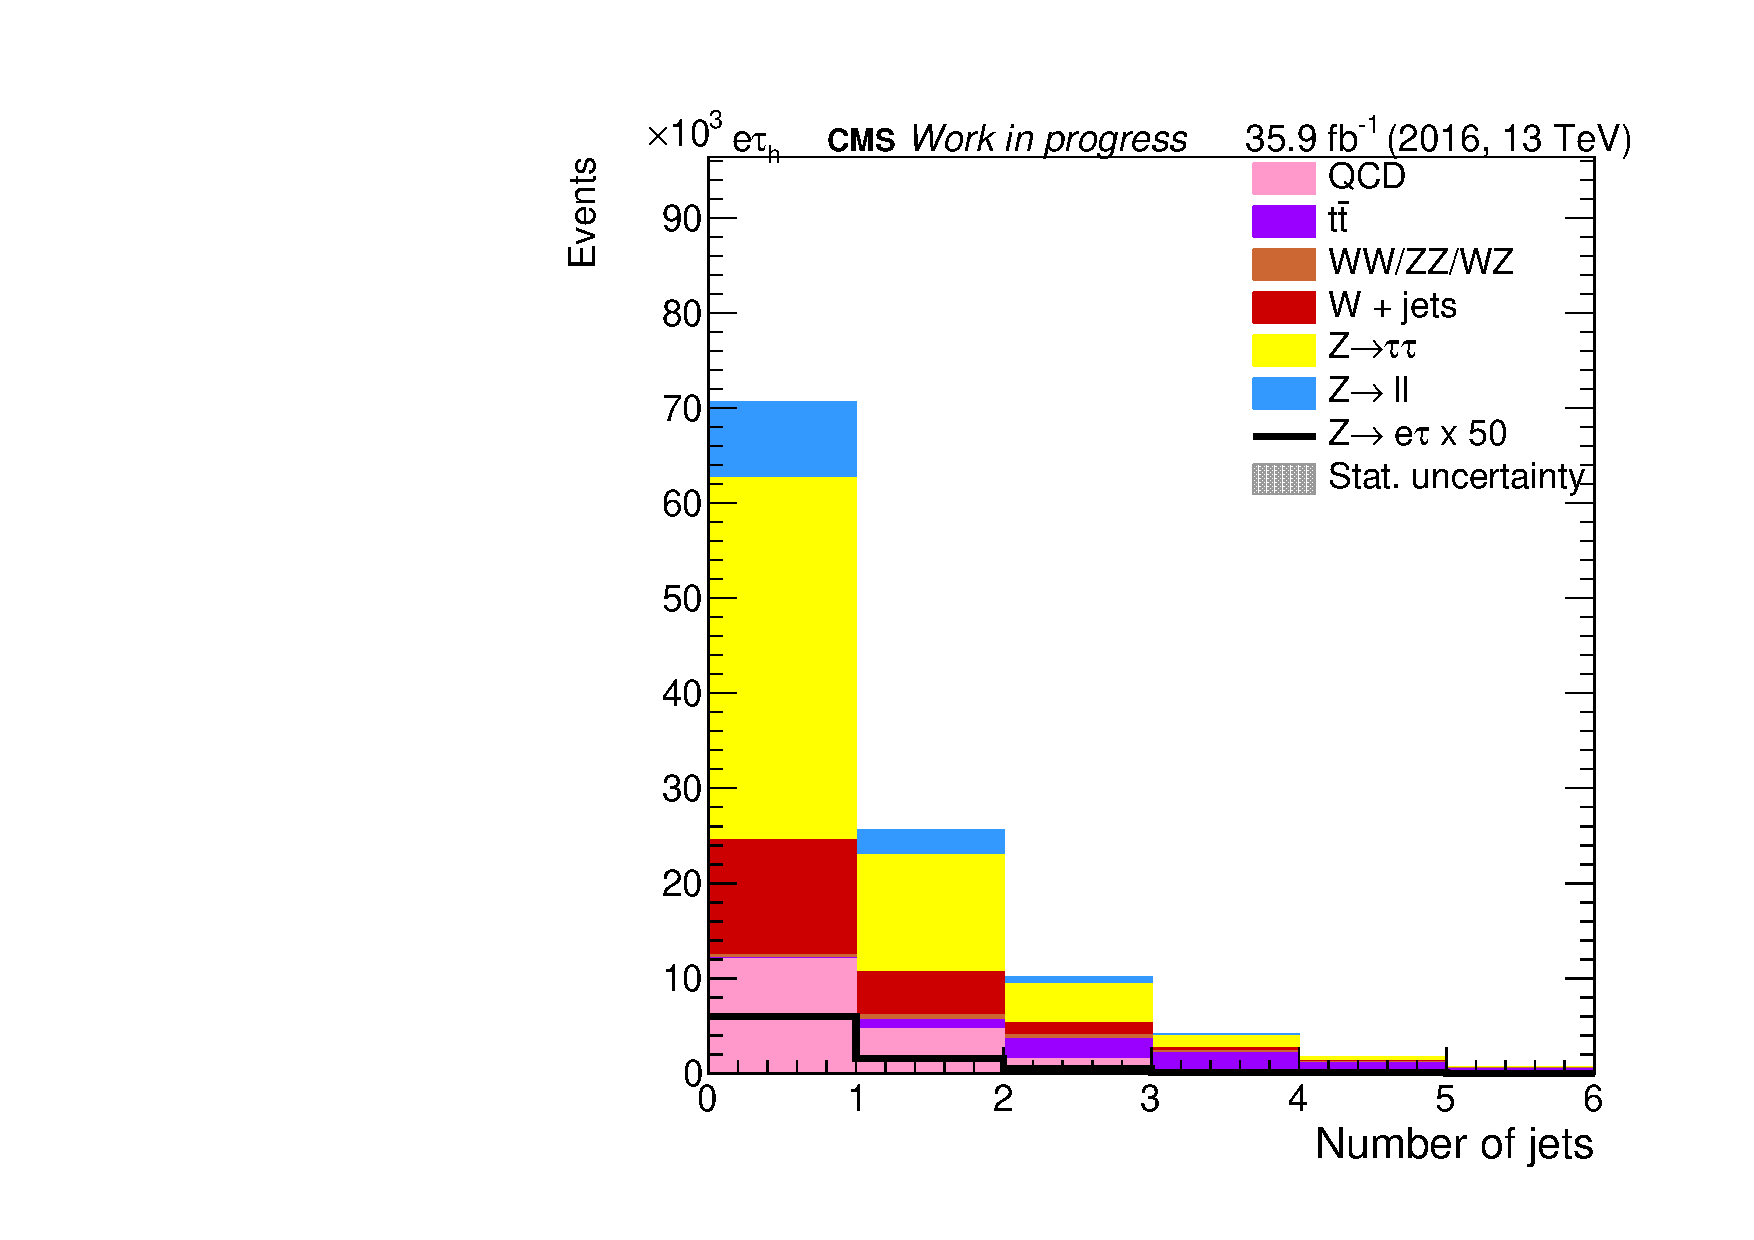
\includegraphics[width=0.55\textwidth]{plots/et/NumberOfJets.pdf}
	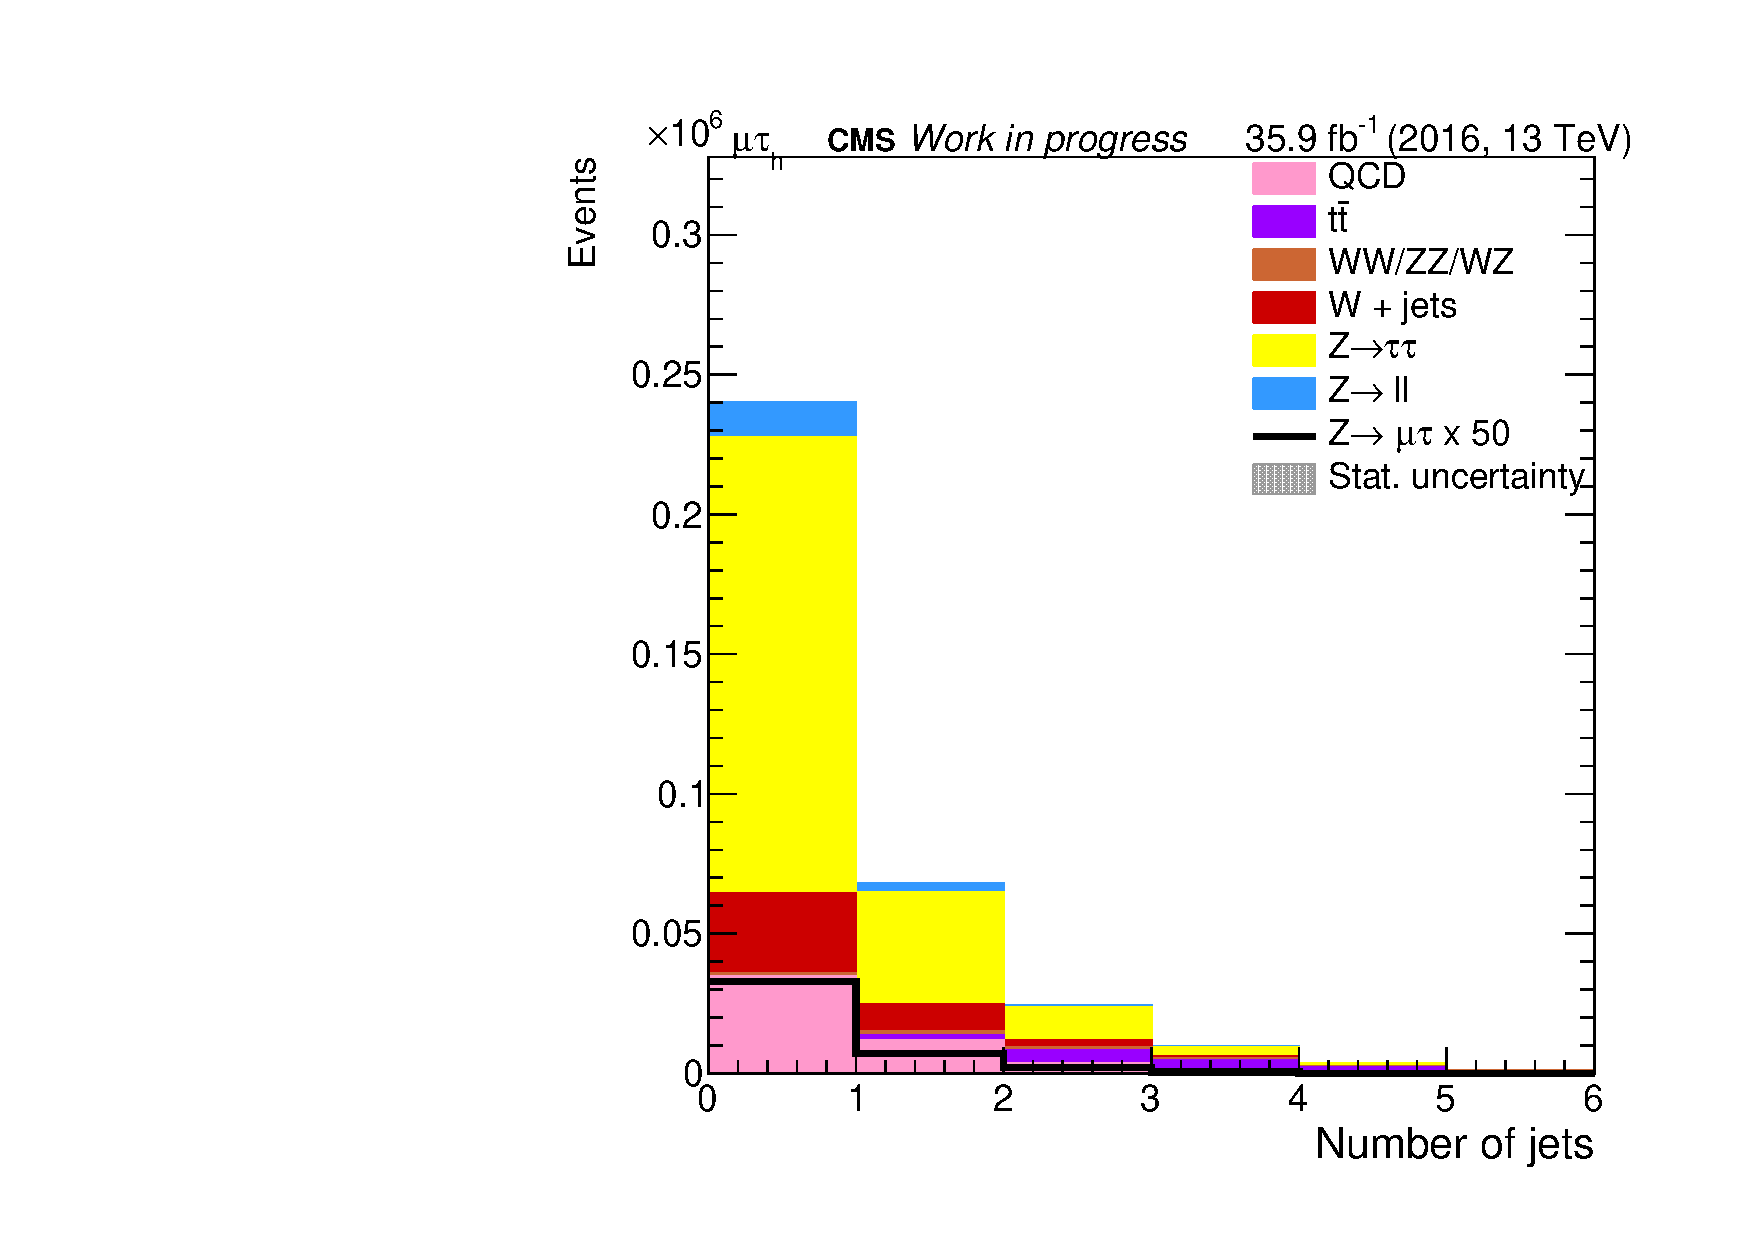
\includegraphics[width=0.55\textwidth]{plots/mt/NumberOfJets.pdf}

	\caption[Number of jet distribution of each final state]{Number of jet distribution for the final state $e\mu$, $e\tau$ and $\mu\tau$}
	\label{fig:fig_3_7}
\end{figure}

For the categorization a cut on the jets multiplicity is applied. Three distinguished regions in phase space are considered:

\begin{description}
	\item [Zero Jet category:] Event with zero jets
	\item [One Jet category:] Event with one jet
	\item [Multi Jet category:] Event with more than one jet
\end{description}


\section{Signal expectation}
\label{sec:section_3_3}

The analysis uses a model independent approach for modelling the signal. This means no theoretical prediction of the branching ratios $\text{BR}(Z\to\text{LFV})$ is given like in the case of \gls{LFV} induced by neutrino oscillation, see section \ref{sec:section_1_3_2}. For this reason the signal expectation is constructed by using information of previous analyses, as discussed in section \ref{sec:section_1_3_3}. The previous analysis set limits on the branching ratios for \gls{LFV} process $\text{BR}(Z\to\text{LFV})$ in each final state, and using this information the signal expectation in this analysis is  set to be

\begin{equation}
	\label{eq:eq_3_3}
	N_{\text{LFV}} = \mathcal{L}_{int} \cdot \sigma(pp\to Z) \cdot \text{BR}(Z\to\text{LFV}), \quad \text{LFV} \in (e\mu, e\tau, \mu\tau)
\end{equation}

with the integrated luminosity $\mathcal{L}_{int}$ and the production cross section for Z bosons at proton-proton collisions $\sigma(pp\to Z)$. Because the $\text{BR}(Z\to\text{LFV})$ is an upper limit for each final state, $N_{\text{LFV}}$ can be interpreted as maximal number of events, which can be expected. \\

The three possible decays of the Z boson into \gls{LFV} are analysed independently, which means that for only the final state of interest a non-vanishing branching ratio is assumed. For example the analysis of the $e\mu$ final state assumes a $\text{BR}(Z\to e\mu) > 0$ and  $\text{BR}(Z\to e\tau) = \text{BR}(Z\to \mu\tau) = 0$. 


\section{Background estimation}

The study of both signal and background processes requires the study of simulations, which can be compared with data. The simulation of the processes are provided by the \gls{CMS} collaboration and are done in three steps. The first is the simulations of the physical process by using a \gls{MC} event generator, for example like Madgraph \cite{MADGRAPH}, which generates mother, daughter particles and their four momenta. The second step is the simulation of proton-proton collisions, including the information of the generated particles. In the last step the detector response of \gls{CMS} is simulated by Geant4 \cite{GEANT4} using the proton-proton and the process simulation. \\

In this simulation the physical expectation for the number of events, given by formula \ref{eq:eq_2_2}, is not included yet. This expectation is determined with the background estimation for each process.

\subsection{Background estimated from Monte Carlo simulation}
\label{sec:section_3_4_1}

To determine background from Z boson decays, \gls{MC} simulation is used and normalized to the cross section and integrated luminosity according to equation \ref{eq:eq_2_2}. It is split into two contributions due to different decay modes of the Z. The first contribution is the $Z\to\tau\tau$ background, where depending on the decay mode of the $\tau$ lepton, \gls{TAUH} are matched to generated hadronic taus and electrons/muons are matched generated leptonic decaying taus. The second contribution is the $Z\to\ell\ell$ background, which combines events where \gls{TAUH} is matched to a generated electron/muon or not matched at all. \\ 

The $t\bar{t}$ and the di-boson background, including all production modes of two vector bosons, top quark in association with a W boson and single top production, is simulated with \gls{MC} and normalized to its cross section and the integrated luminosity. 


\subsection{Background estimated using data driven methods}
\label{sec:section_3_4_2}

For the $e\mu$ final state, $W + \text{jets}$ is a minor background due to the small probability for a jet to be misidentified as an isolated lepton. Because of this, in this final state the estimation is done with \gls{MC} simulation and normalized with cross section and integrated luminosity. The \gls{QCD} shape is taken from a region, where both leptons have the same charge (same-sign region) and pass relaxed isolation criteria. The normalization is extrapolated from comparing same-sign (SS) and opposite-sign (OS) regions, where one of the two leptons fulfil $0.3 < I^{\ell} < 0.5$.  \\

In the case of the $e\tau$ / $\mu\tau$ final state, $W + \text{jets}$ normalization and \gls{QCD} is simultaneously estimated with a data driven method. The number of events in the OS signal region (SR), where events fulfil $M_T < 50$ GeV (low $M_T$), is calculated with 

\begin{equation}
	W^{\text{low } M_T}_{OS} = \Bigg(\frac{W^{\text{low } M_T}_{\text{sim. relaxed OS}}}{W^{\text{high } M_T}_{\text{sim. relaxed OS}}}\Bigg) \cdot W^{\text{high } M_T}_{OS}
\end{equation}

with $W^{\text{low } M_T}_{\text{sim. relaxed OS}}$ and $W^{\text{high } M_T}_{\text{sim. relaxed OS}}$ as number of events taken from simulation, where relaxed isolation criteria is applied. For the number of events in the OS region in the control region (CR), where events fulfil $M_T > 50$GeV (high $M_T$), is extracted from data using 

\begin{equation}
	W^{\text{high } M_T}_{OS} = \text{data}^{\text{high } M_T}_{OS} - Z^{\text{high } M_T}_{OS} - t\bar{t}^{\text{high } M_T}_{OS} - \text{diboson}^{\text{high } M_T}_{OS} - \text{QCD}^{\text{high } M_T}_{OS}
\end{equation}

with data and all other backgrounds explained in the previous section. The number of events for QCD in the high $M_T$ region with OS events are estimated using

\begin{equation}
\text{QCD}^{\text{high } M_T}_{OS} = \epsilon^{QCD}_{OS/SS} \cdot (\text{data}^{\text{high } M_T}_{SS} - Z^{\text{high } M_T}_{SS} - t\bar{t}^{\text{high } M_T}_{SS} - \text{diboson}^{\text{high } M_T}_{SS} - W^{\text{high } M_T}_{\text{sim. SS}})
\end{equation}

with simulated $W + \text{jets}$ events, in the SS high $M_T$ CR region. The factor $\epsilon^{QCD}_{OS/SS}$ is an extrapolation from SS to OS region, which is calculated using samples with inverted isolation criteria of the leptons. Using the same extrapolation factor, the distribution of QCD in the low $M_T$ signal region is calculated using 

\begin{equation}
	\text{QCD}^{\text{low } M_T}_{OS} = \epsilon^{QCD}_{OS/SS} \cdot (\text{data}^{\text{low } M_T}_{SS} - Z^{\text{low } M_T}_{SS} - t\bar{t}^{\text{low } M_T}_{SS} - \text{diboson}^{\text{low } M_T}_{SS} -  \Bigg(\frac{W^{\text{low } M_T}_{\text{OS}}}{W^{\text{high } M_T}_{\text{sim. OS}}}\Bigg) \cdot W^{\text{low } M_T}_{\text{SS}})
\end{equation}


\subsection{Correction of simulated events}
\label{sec:section_3_4_3}

Limited power of modelling the proton-proton-interactions, pile up and the detector response leads to discrepancies between the \gls{MC} simulation and data. To correct such discrepancies, scale factors and kinematic corrections are applied. In general the factors for the corrections are provided by the \gls{CMS} collaboration. \\

Trigger and identification of particles shows different efficiencies in data and \gls{MC}. With scale factors binned in \gls{pT} and \gls{eta}, these efficiencies of \gls{MC} are matched to data. For the identification the scale factors depend on the working point of the identification selection. For the case of the \gls{TAUH}, where extra \gls{MVA} identifications to discriminate electrons and muons are used, scale factors in bins of \gls{eta} are applied. \\

Besides selection efficiencies, corrections on the measured energy/momentum have to be applied. In the case of the \gls{TAUH}, the four momenta is corrected by -1.8\% in the 1-prong decay mode, by +1.0\% in the 1-prong + $\pi^{0}$ decay mode and by 0.4\% in the 3-prong decay mode. To correct the energy scales of electrons/muons faking a \gls{TAUH} the four momentum of \gls{TAUH}, which are matched on generator level to an electron or muon, are corrected. For matched \gls{TAUH} to a muons a correction of -0.2\% for the 1-prong decay mode and of +1.5\% for the 1-prong + $\pi^{0}$ decay mode is applied. For matched \gls{TAUH} to an electron a correction of 9.5\% in the 1-prong + $\pi^{0}$ decay mode is applied. \\

For the jet energy scale factors on the jet four momenta are applied. The \gls{MET} is corrected by a propagating the jet energy corrections through the calculation of the MET. For the Z boson and top quark, \gls{pT} corrections are applied. \\

For the $Z\to\tau\tau$ process, scale factors are calculated from a $Z\to\mu\mu$ control sample, where 2D scale factors in \gls{pT} and \gls{m_vis} are calculated like in the SM $H\to\tau\tau$ analysis \cite{SMHTT}. For the corrections of \gls{TTBAR}, scale factors depending on the generated top \gls{pT} are applied.


\section{Discriminating variable}
\label{sec:section_3_5}

The goal of the analysis is to find a excess in data, which could indicate \gls{LFV}. To find an excess, which is not covered by statistical/systematic uncertainties of the background simulation, a discriminating variable has to be chosen for the analysis, which separates the signal and background processes. In general two approaches can be studied. The first approach is a cut-based strategy, in which a set of sensitive parameters are chosen, then cuts are applied on these parameters to enhance the signal/background ratio, while keeping enough events for a sufficient statistical analysis. The second approach are the usage \gls{MVA} classifier, as already introduced in the identification of leptons in section \ref{sec:section_3_2_2}. The \gls{MVA} classifier is trained on events, where the classification is already known (signal or background), and then is later applied on events with unknown classification. 

\subsection{Boosted decision tree}
\label{sec:section_3_5_1}

A boosted decision tree (\gls{BDT}) \cite{BDT} is a continuous binary \gls{MVA} classifier, which can distinguish between two kind of sets, which can be classified. In the case of this analysis, one set is the collection of all backgrounds, and the second set is the \gls{LFV} signal. For each final state independently, a \gls{BDT} classifier is trained to discriminate between the collection of all backgrounds and the signal. \\

The boosted decision tree is an iteration of the many decision trees (\gls{DT}). Figure \ref{fig:fig_3_10} shows the schematic overview which is explained in the following. A set of $N_{events}$ events, where each event $j$ has a event weight $w_{j}$ and a tuple of parameters $x = (x_{1}, ... , x_{i})$ with $i \in \mathbb{N}$, is given as the input of the \gls{DT}. The events have a known labelling, for example background (B) and signal (S). For the set the signal purity is defined as

\begin{equation}
	\label{eq:eq_3_10}
	P = \frac{\sum_{j \in (\text{signal events})} w^{j}}{\sum_{j \in [1, N_{events}]} w^{j}}.
\end{equation}

From the parameter tuple $x$ the parameter $x_{i}$ and the cut value are chosen, which gives the best separation of the samples, which is quantified for example by the gini index 

\begin{equation}
	\label{eq:eq_3_11}
	g = \sum_{j \in [1, N_{events}]} w^{j} \cdot P \cdot (1-P).
\end{equation}

The set is split into two subsets, one having a higher signal purity, while the other subset is higher background purity. On these subsets the same procedure is followed, until the stop condition is hit (maximal number of iterations, minimal numbers of events in a subset, perfect signal/background separation). The events are labelled by the \gls{DT} according the last subset, they land in. This gives a non-continuous binary classification of each event by the \gls{DT}. \\

\begin{figure}[htp]
	\centering
	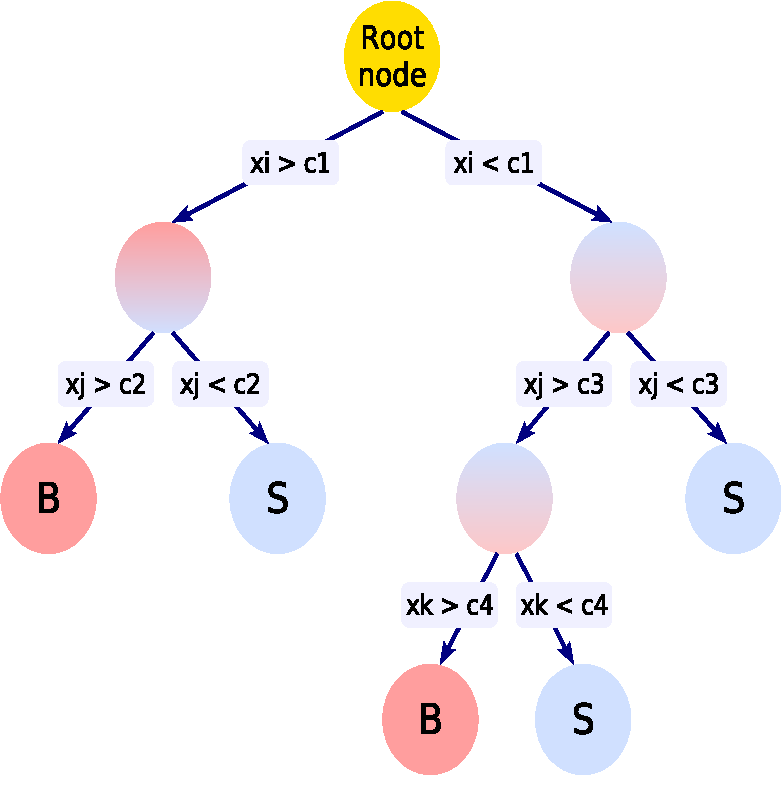
\includegraphics[width=0.7\textwidth]{pictures/DT.pdf}

	\caption[DT scheme]{Scheme of a generic decision tree, taken from \cite{TMVA}}
	\label{fig:fig_3_10}
\end{figure}


In the algorithm of the \gls{BDT} $N_{T}$ \gls{DT} are trained and incorrectly classified events are re-weighted. For each decision tree \gls{DT} $k$ the event $j$ has weight $w^{j}_{k}$. After the $k^{\text{th}}$ \gls{DT} training the misidentification probability is calculated with

\begin{equation}
	\epsilon_{k} = \frac{\sum_{j}^{N_{events}} w^{j} \cdot \text{isMisidentified}(j)}{\sum_{j}^{N_{events}} w^{j}}.
\end{equation}

For the next \gls{DT} all misclassified events are re-weighted with $w^{j}_{k+1} = w^{j}_{k} \cdot e^{\alpha_{k}}$ with $\alpha_{k} = \beta \cdot \ln{\frac{1-\epsilon_{k}}{\epsilon_{k}}}$ and $\beta$ as learning rate, which gives misclassified events a higher impact of decisions of the set splitting. To quantify the result of the iterations of all \gls{DT}, a continuous parameter, the so-called BDT score, is defined as 

\begin{equation}
	\label{eq:eq_3_12}
	T(j) = \frac{1}{\sum_l^{N_T} \alpha_k} \sum_k^{N_T} \alpha_k \cdot T_k(j)
\end{equation}

with $T_k(j)$ as the binary output of the $k^{\text{th}}$  decision tree. The BDT score is constructed in a way, that is ranges from -1 to 1. In case of the analysis, all signal-like events are bigger than zero and all background-like events are smaller than zero. 


\subsection{Training and application}
\label{sec:section_3_5_2}

The \gls{BDT} algorithm explained in section \ref{sec:section_3_5_1} has a set of free tunable parameters, which is called hyperparameter space. The hyperparameters influence the performance of the training and are tuned to give the best separation between background and signal. In this analysis the choice for the hyperparameters are:

\begin{itemize}
	\item Number of decisions trees: 800
	\item Maximal number of iteration in a decision tree: 4
	\item Minimum number of events in a subset: $0.025 \cdot N_{events}$
	\item Learning rate: 0.1
\end{itemize}

The events, on which the training is performed, are taken from the \gls{MC} simulation of all backgrounds and the \gls{LFV} signal that pass the event selection, which is discussed in section \ref{sec:section_3_2_2}. The initial weights are chosen according the physical expectation discussed in the section \ref{sec:section_3_4_1} of the background estimation. For the \gls{QCD} multijet, which is estimated from data driven techniques, no events can be used for the training. Under the assumption, that the \gls{QCD} events in data are labelled as background-like in a \gls{BDT},  the training is performed without \gls{QCD} information. \\

The properties of signal and background processes are reflected in the kinematic distributions of the leptons and the reconstructed Z boson. Because of this, the parameter tuple $x$ includes

\begin{description}
	\item [Angular correlations:] $\Delta \phi(\ell_1, \ell_2)$, $\Delta \phi(\ell_1, {E}_{T})$, $\Delta \phi({E}_{T}, \ell_2)$, $\Delta \phi(\ell_1, Z)$, $\phi(Z, \ell_2)$, $\Delta \theta(\ell_1, \ell_2)$
	\item [Lepton properties:] $p_T(\ell_1)$,  $p_T(\ell_2)$, $|d_0(\ell_1)|$, $|d_0(\ell_2)|$, $m_T(\ell_2)$
	\item [Reconstructed $Z$ boson properties:] $p_T(Z)$, $m_T(Z)$, $E(Z)$, $m_{vis}$, ${E}_{T}$
\end{description}

The plots of all parameter are shown in appendix \ref{sec:appendix_A}. \\

For the training of the \gls{BDT} the TMVA software package \cite{TMVA} is used. The different final state is trained independently from each other. For each final state, two trainings are performed. The training events of the \gls{MC} simulation are split into even-numbered and odd-numbered event sets. The odd-numbered set is used for the training of the \gls{BDT} classifier, and is then applied on the even-numbered set for data and \gls{MC}, and vice versa. This procedure enables the use of the complete \gls{MC} events without statistical biases. 

\subsection{BDT output}
\label{sec:section_3_5_3}

The trained \gls{BDT} assigns the \gls{BDT} score to each event according to formula \ref{eq:eq_3_12}. The \gls{BDT} score is then used as the discriminating variable for the statistical analysis described in section \ref{sec:section_5_1}. Figure \ref{fig:fig_3_11} shows the inclusive distribution of the \gls{BDT} score and a unblinded signal-free \gls{BDT} score distribution each final state. \\

 
\begin{figure}[htp]
	\centering

	\begin{multicols}{2}
		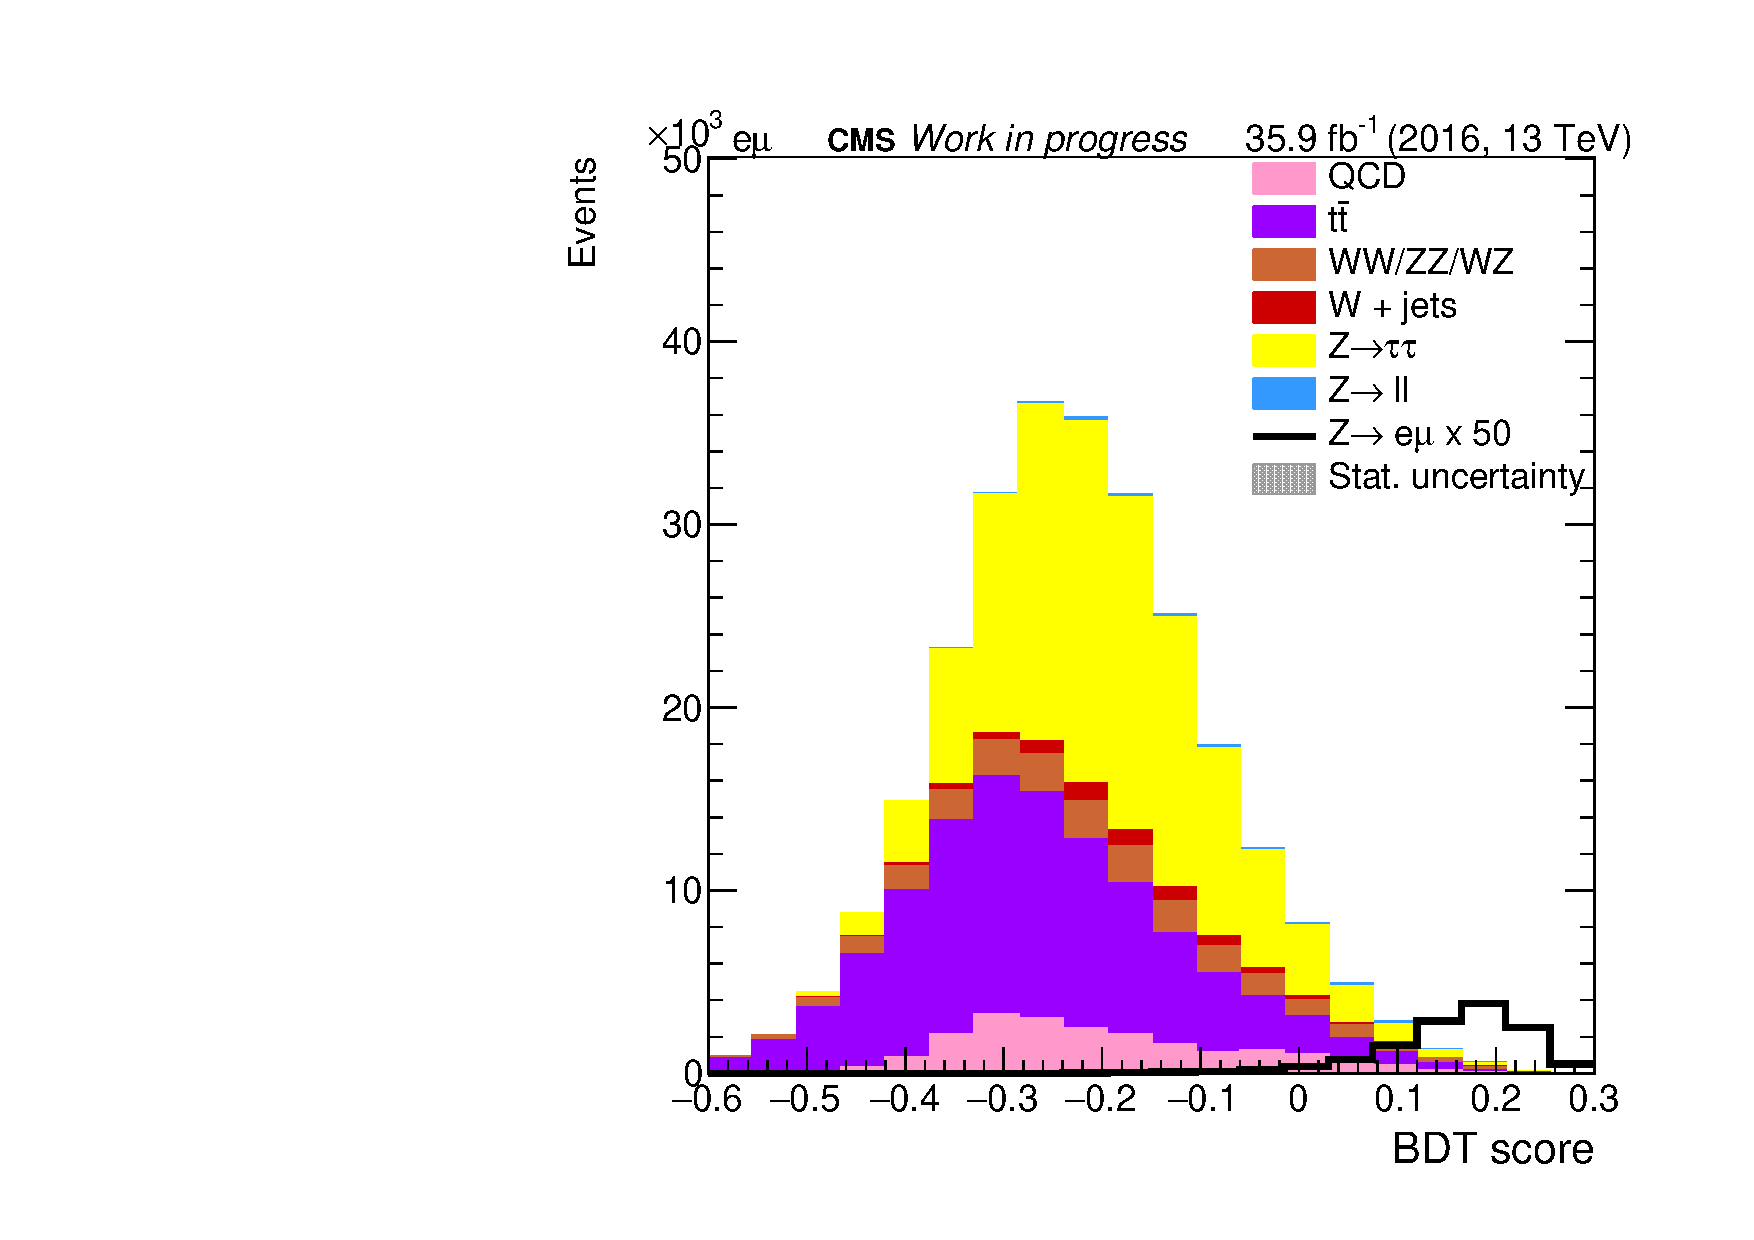
\includegraphics[width=\linewidth]{plots/em/BDTScore.pdf}\par 
		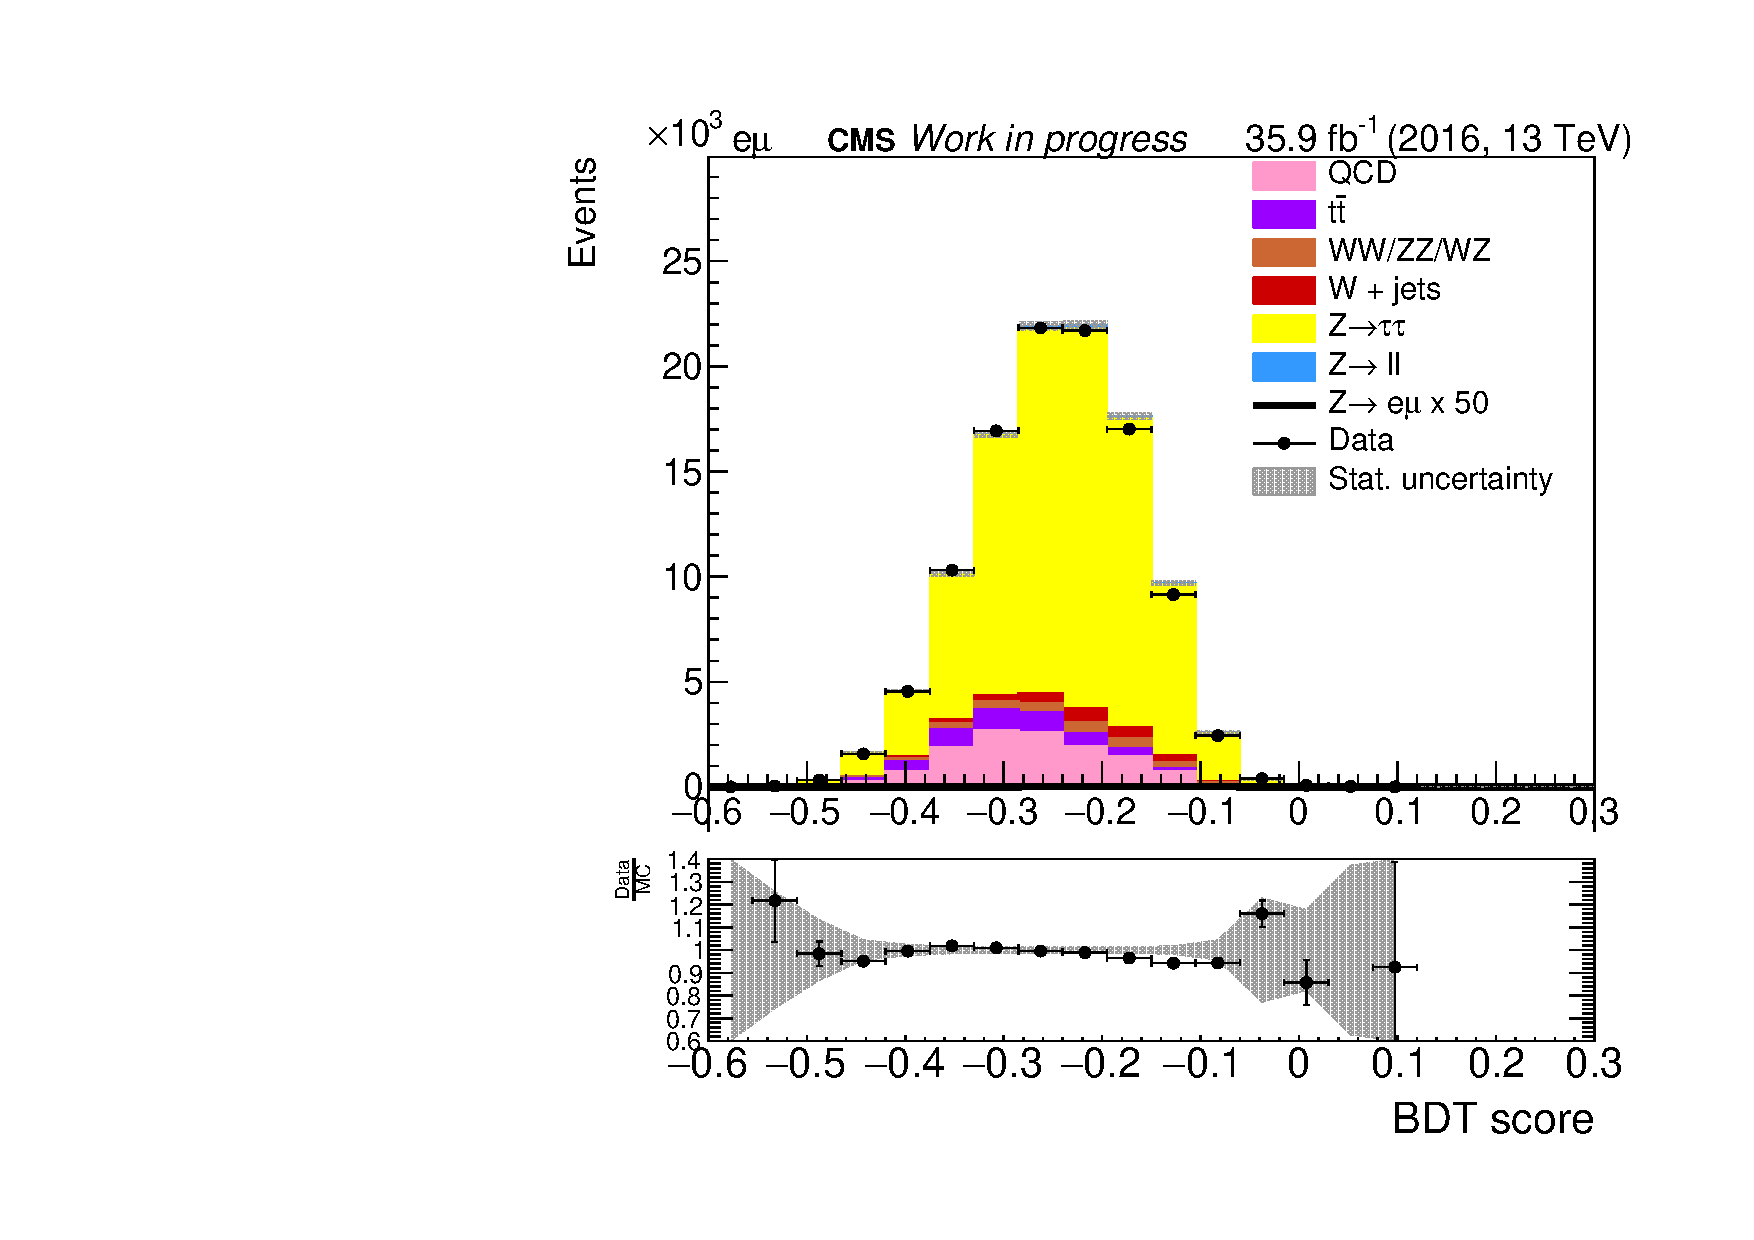
\includegraphics[width=\linewidth]{plots/em/BDTScore_ZTTCR}\par
	\end{multicols}

	\begin{multicols}{2}
		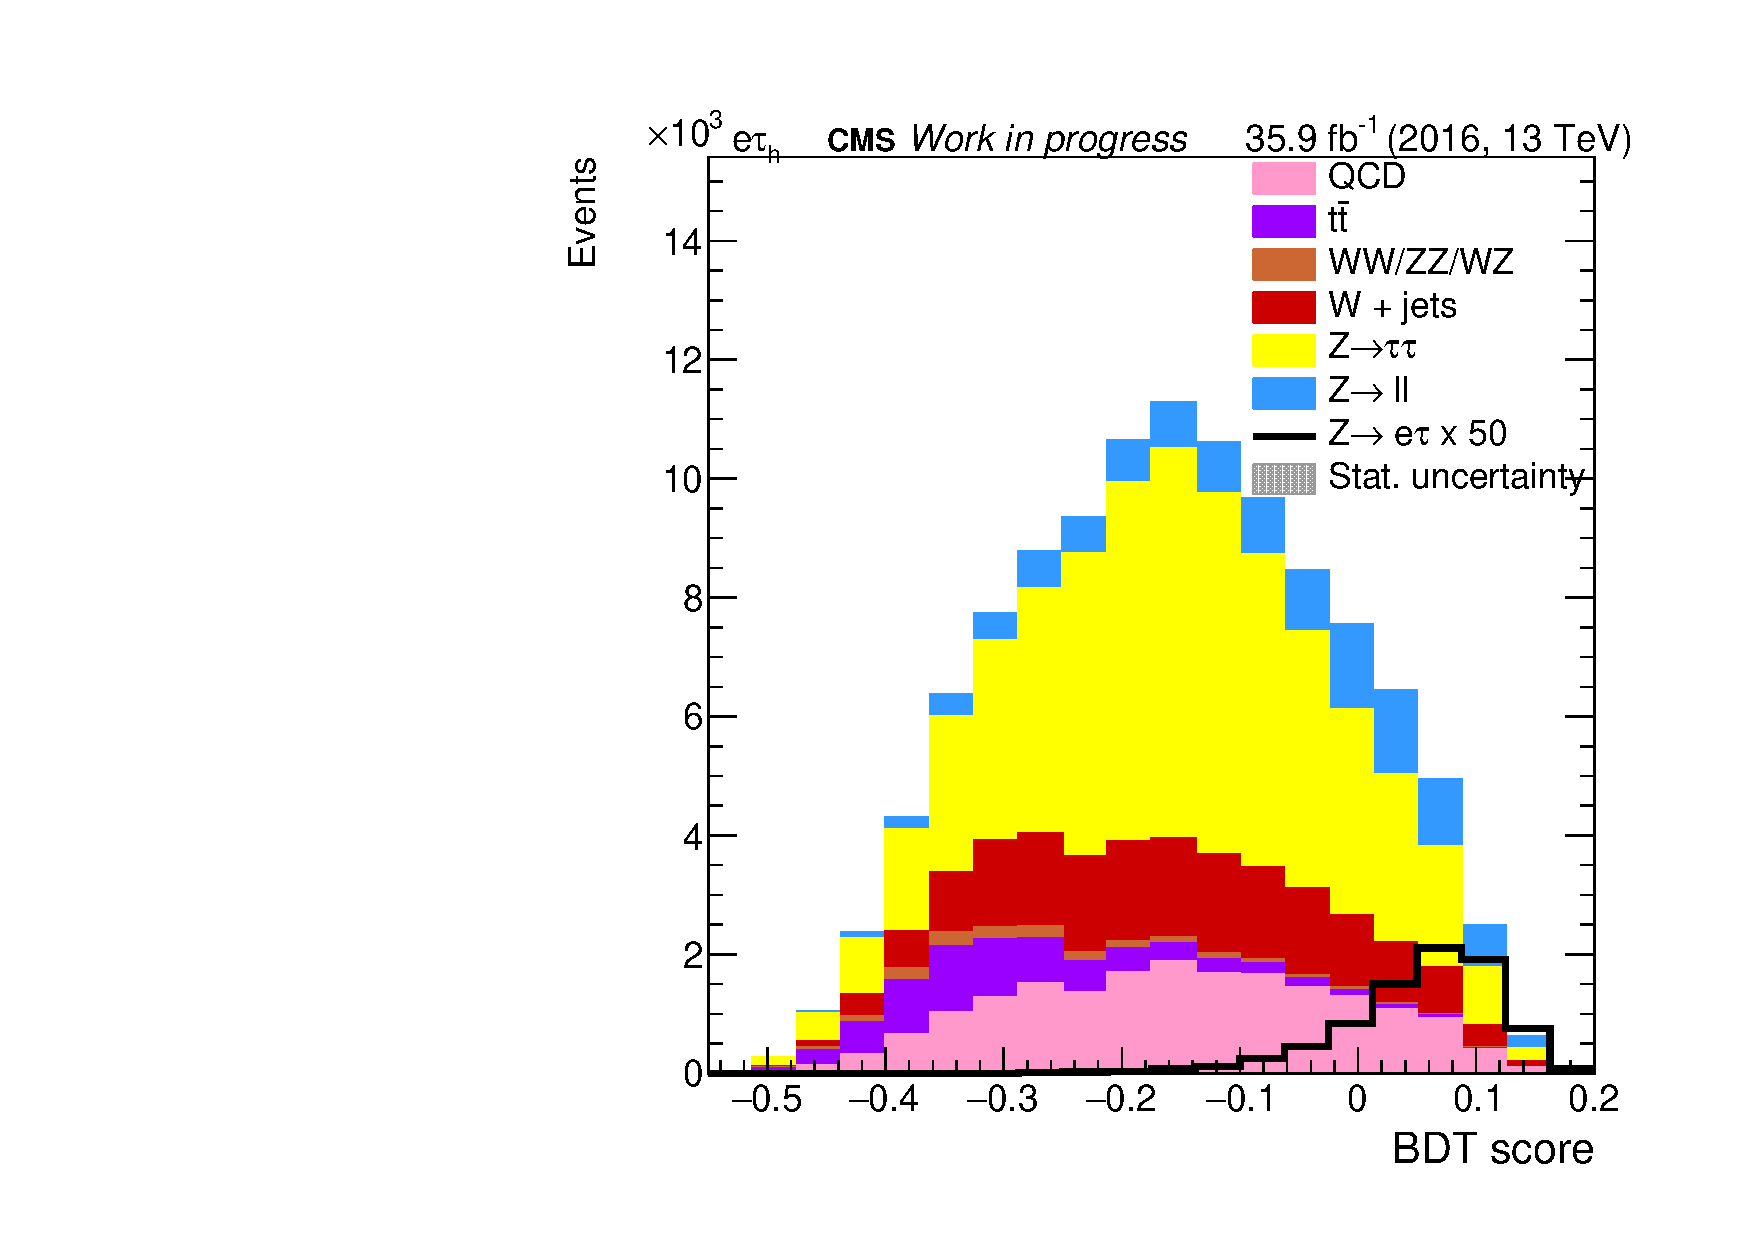
\includegraphics[width=\linewidth]{plots/et/BDTScore.pdf}\par 
		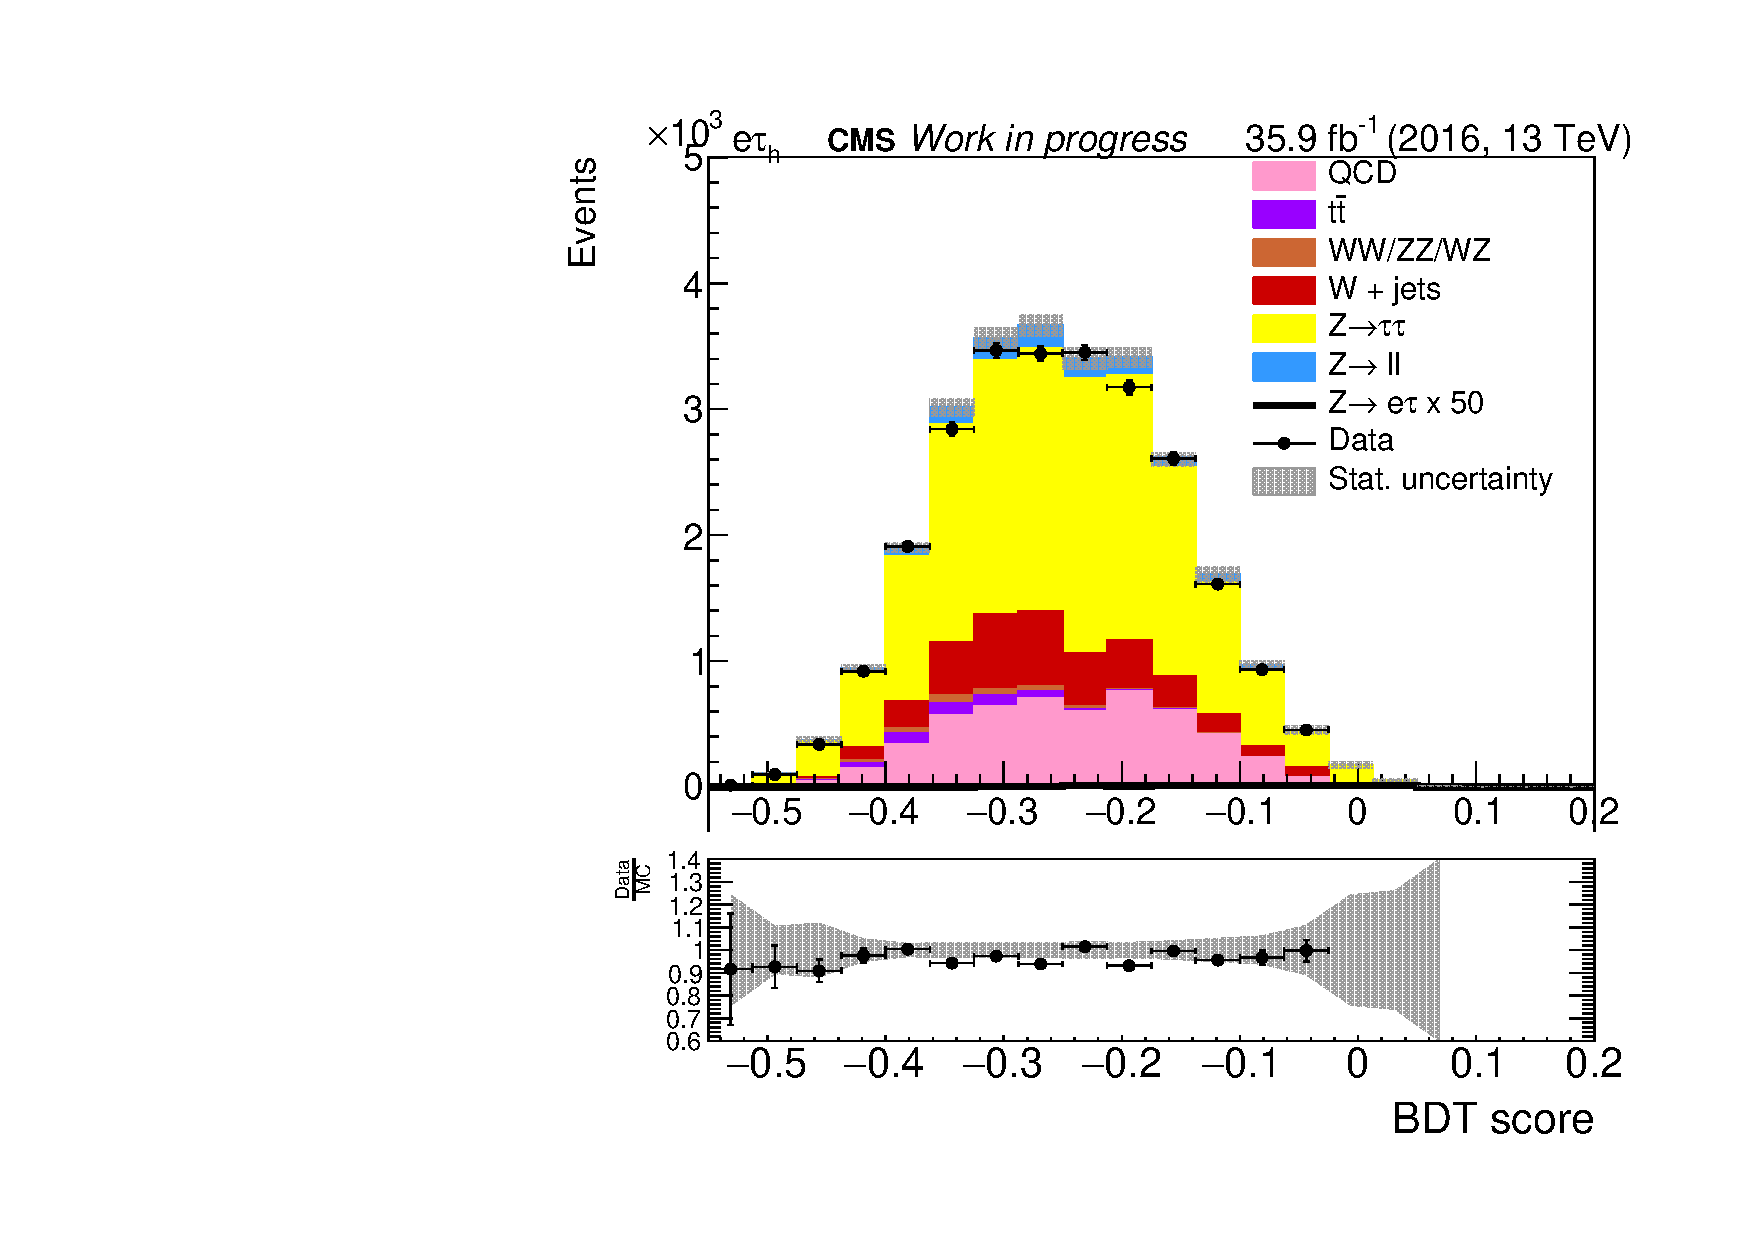
\includegraphics[width=\linewidth]{plots/et/BDTScore_ZTTCR}\par
	\end{multicols}	

	\begin{multicols}{2}
		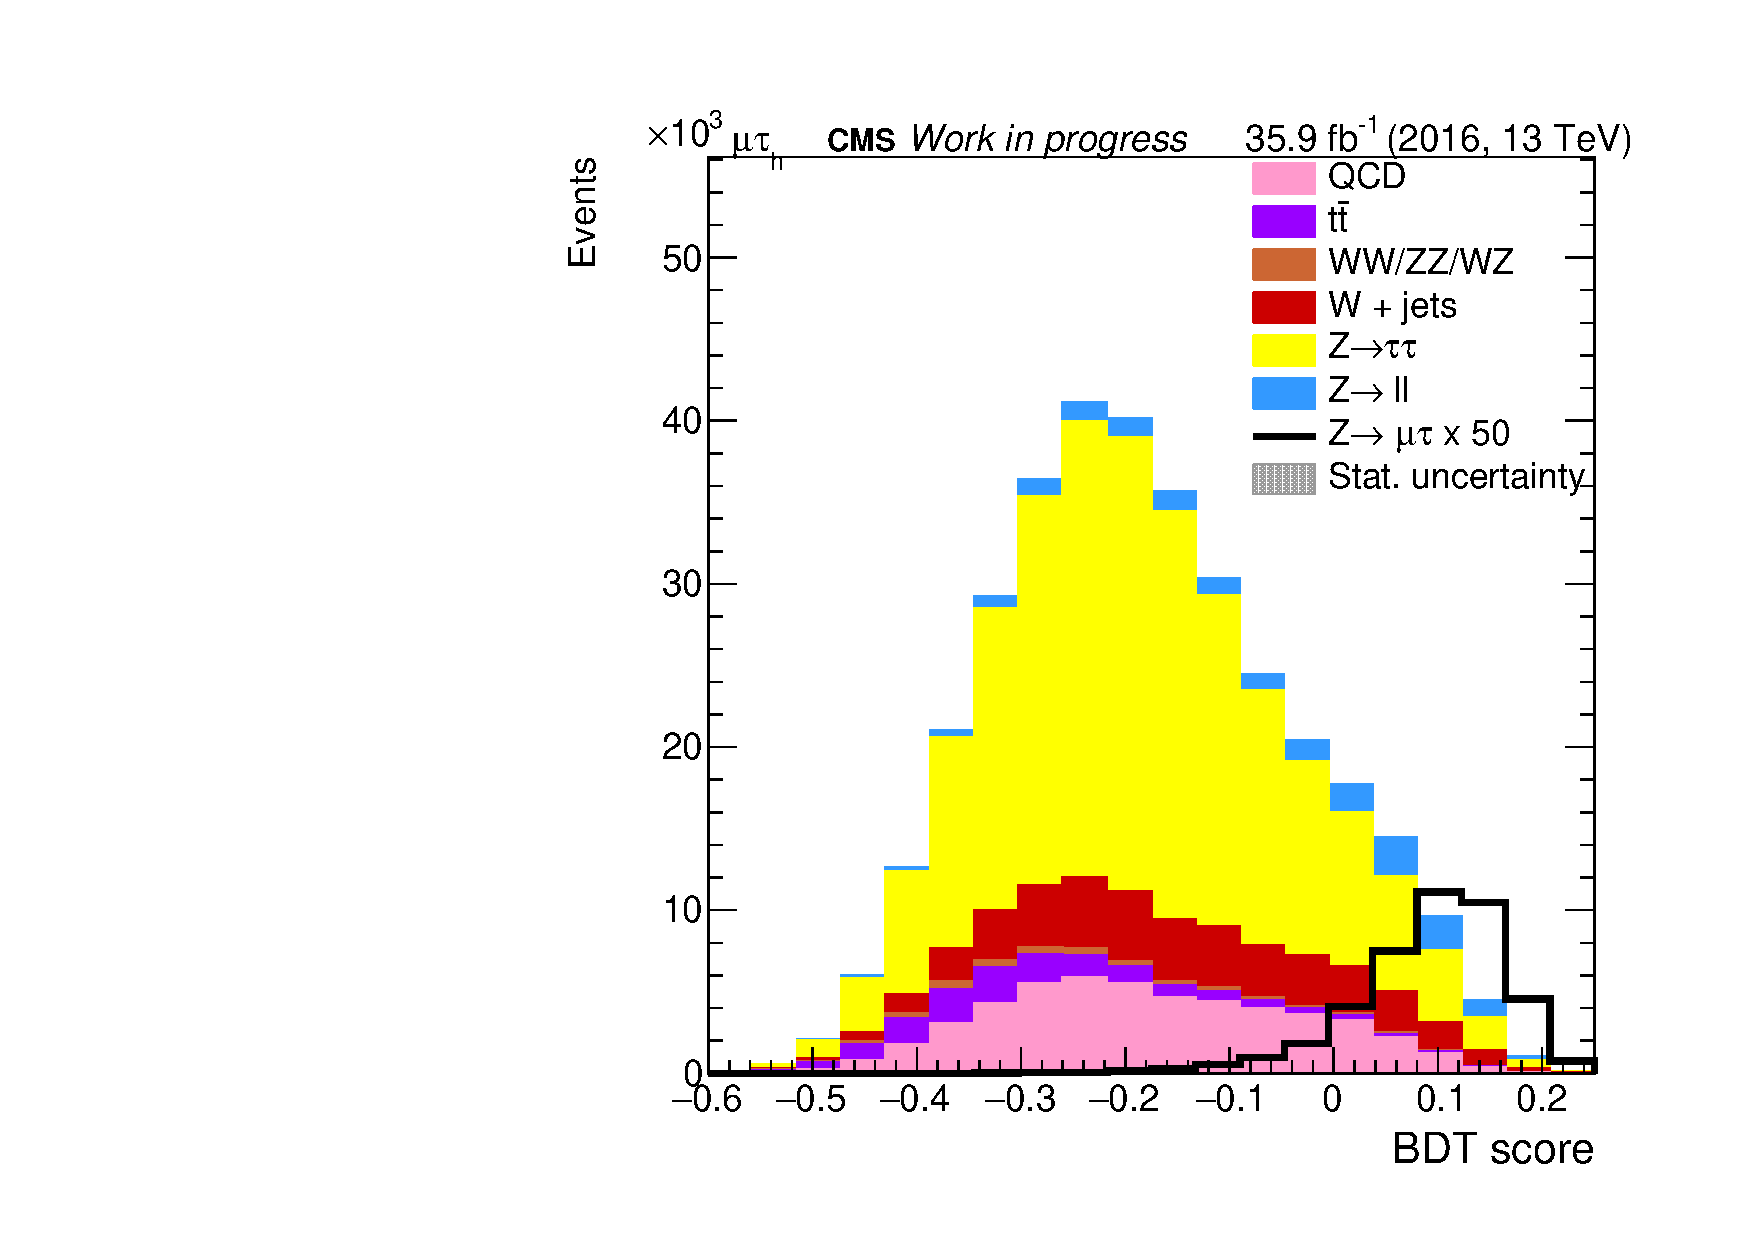
\includegraphics[width=\linewidth]{plots/mt/BDTScore.pdf}\par 
		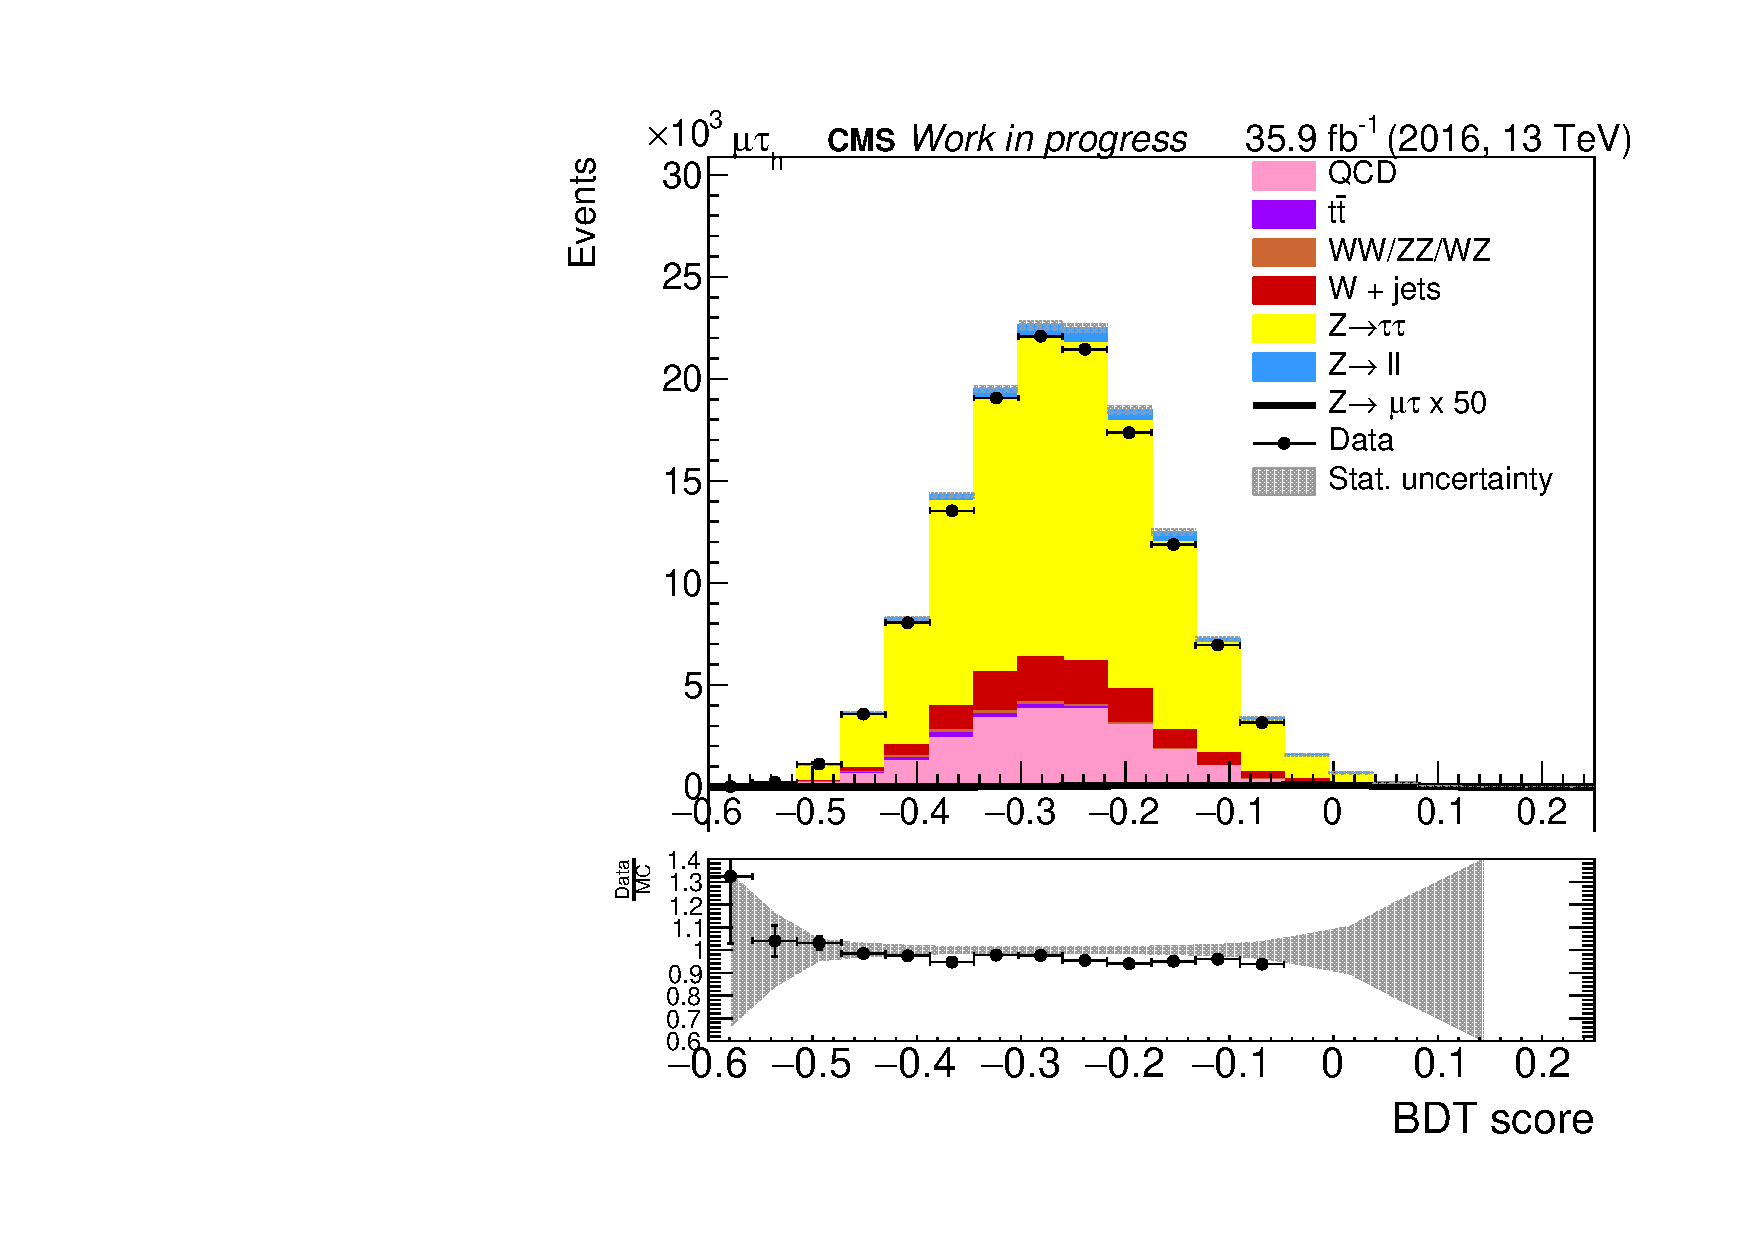
\includegraphics[width=\linewidth]{plots/mt/BDTScore_ZTTCR}\par
	\end{multicols}		

	\caption[BDT score]{\gls{BDT} score for the final state $e\mu$, $e\tau$ and $\mu\tau$, one the left inclusive plots with signal, on the right signal free unblinded plots with events \gls{m_vis} $< 60$ GeV and a ratio plot of \gls{MC} and data with the grey band as statistical uncertainty}
	\label{fig:fig_3_11}
\end{figure}

For the $e\mu$ final state the \gls{BDT} score shows a well separation of background and signal, for the $e\tau$ and $\mu\tau$ final state the discrimination power of the \gls{BDT} score is lower. The difference in separation power is caused by the challenge of the reconstruction of \gls{TAUH}. In the $e\mu$ final state, both leptons are prompt, well isolated and in events of the signal no neutrinos are involved. This is reflected in the kinematic distributions of this final state, which have already quite separation power by itself. In the $e\tau$ and $\mu\tau$ final state the reconstruction of the \gls{TAUH} is more challenging than the reconstruction of the electron or muon, and gives rise to more uncertainties to deal with. This is reflected in the separation power of distributions of the kinematic parameter, and therefore also in the \gls{BDT} score. 










	

































